\documentclass[11pt,a4paper]{article}

\usepackage[utf8]{inputenc}
\usepackage[english]{babel}
\usepackage[T1]{fontenc}
\usepackage{graphicx}
\usepackage{bm}
\usepackage[colorlinks=true]{hyperref}


\usepackage{amsmath,amssymb,amsfonts,amsthm}
\newcommand{\mbf}[1]{\bm{#1}}

\title{Assignment 2}
\author{Sebastian Paaske Tørholm \& Kristoffer Søholm \& Søren Dahlgaard}

\begin{document}
\maketitle

\section{Question 1.1}
Performing maximum likelihood estimation as described in
\cite[sec. 3.1.1]{Bishop} we achieve an RMS of $4.75$ with the 4-dimensional
data set and an RMS of $5.43$ with the 1-dimensional data set. Based on this
it would seem like the 4-dimensional data set provides ud with better
predictions.

\begin{figure}[h!]
    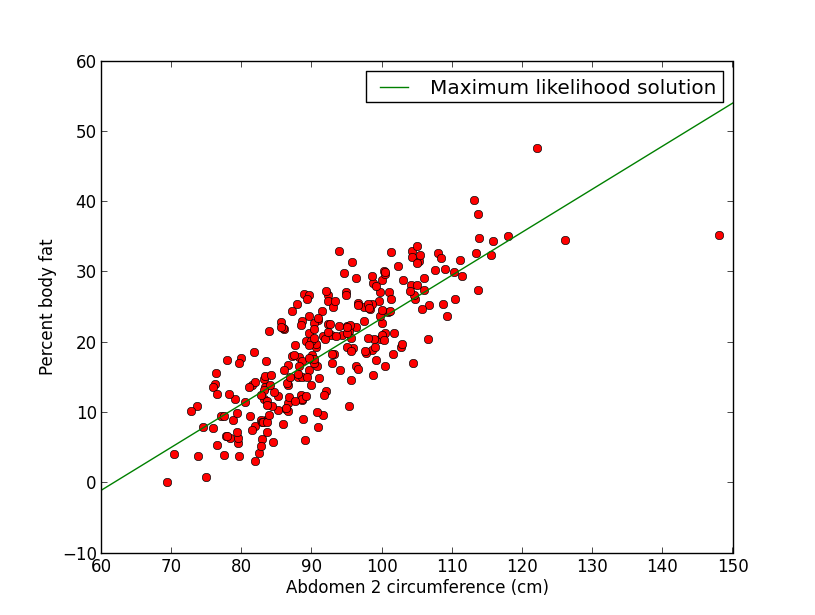
\includegraphics[width=\textwidth]{images/prob11-sel2.png}
    \caption{Maximum likelihood plotted against the combined training \& test points for selection 2}
\end{figure}

\section{Question 1.2}

% 1.2 (MAP) RMS for 4D test set:  4.60495349694
% 1.2 (MAP) RMS for 1D test set:  4.215122148

\begin{figure}[h!]
    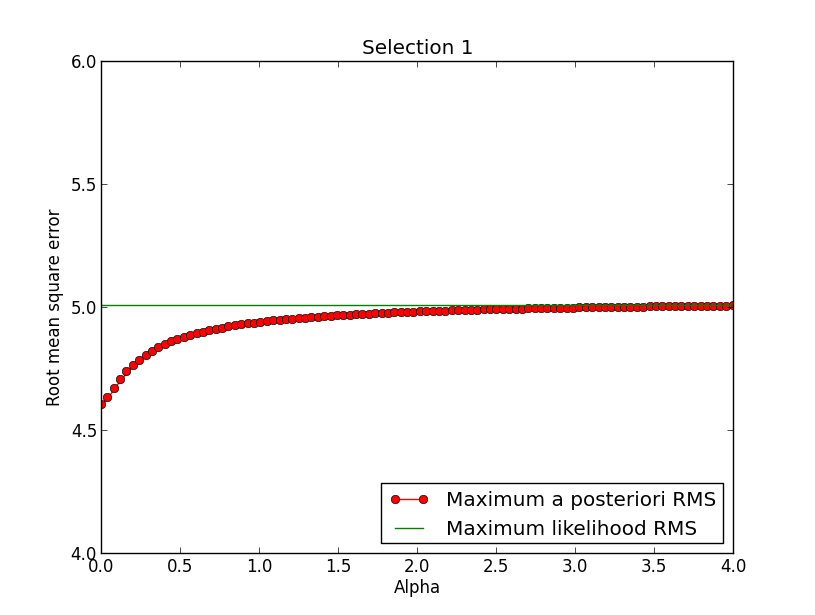
\includegraphics[width=\textwidth]{images/prob12-sel1.png}
\end{figure}
\begin{figure}[h!]
    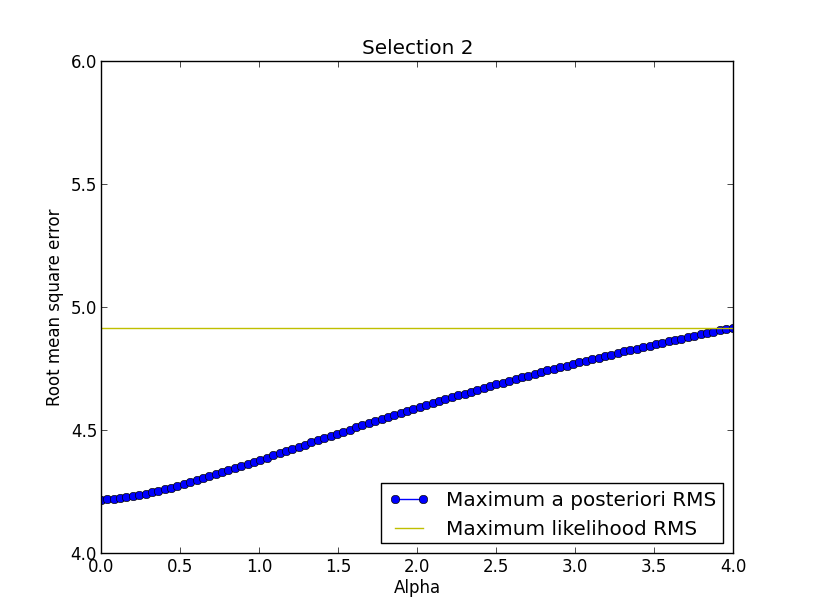
\includegraphics[width=\textwidth]{images/prob12-sel2.png}
\end{figure}



\section{Question 1.3}
We wish to find $p(w|t)$ and know that this is proportional to $p(w)p(t|w)$,
so we ``complete the square'' by looking at the exponential term:
\begin{align*}
    &\exp\left(-\frac{1}{2}(w-m_0)^T S_0^{-1}(w-m_0)\right)
    \prod_{n=1}^N \exp\left(-\frac{\beta}{2}(t_n-w^T\phi(x_n))^2\right)\\
    = &\exp\left(-\frac{1}{2}(w-m_0)^T S_0^{-1}(w-m_0) +
    \sum_{n=1}^N -\frac{\beta}{2}(t_n-w^T\phi(x_n))^2\right)\ .
\end{align*}
By looking at all the terms depending on $w$ in this formula, we can find the
mean and covariance matrix of $p(w|t)$. From the above formula we see, that
these terms are exactly
\begin{align*}
    &-\frac{1}{2}(w^TS_0^{-1}w - 2w^TS_0^{-1}m_0) -\frac{\beta}{2}
    \sum_{n=1}^N \left(-2t_nw^T\phi(x_n) + (w^T\phi(x_n))^2\right)\\
    = &-\frac{1}{2}(w^TS_0^{-1}w - 2w^TS_0^{-1}m_0) -\frac{\beta}{2}\left(
    -2w^T\Phi(x)^T t + w^T\Phi(x)^T\Phi(x)w\right) \\
    = &-\frac{1}{2}(w^TS_0^{-1}w - 2w^TS_0^{-1}m_0)
    +\beta w^T\Phi^T t -\frac{\beta}{2} w^T\Phi^T\Phi w \\
    = &\ w^T(S_0^{-1}m_0 + \beta\Phi^T t) - \frac{1}{2}w^T(S_0^{-1}
    + \beta\Phi^T\Phi)w\ .
\end{align*}
From this we immediately get
\[
    \Sigma^{-1} = S_0^{-1} + \beta\Phi^T\Phi\ ,
\]
and we also know that the linear coefficient of $w$ above is equal to
$\Sigma^{-1}\mu$, so we get
\[
    \mu = \Sigma(S_0^{-1}m_0 + \beta\Phi^t t)\ .
\]
We have now proved eqn.~3.49 of \cite{Bishop}, which is what we wanted to
do.\qed


\section{Question 2.1}
A visualization of the training set can be seen in \autoref{fig:iris_train}.
As can be seen, the yellow class is quite separated from the rest, while the
blue and red class seems very intertwined.

We have chosen to use Fisher's linear discriminant as it is not as susceptible
to problems stemming from outliers, and it handles the in-class variance very
well. We expect, that it should be able to separate the yellow class from the
rest, and perform somewhat reasonable on the red/blue division.

Using the LDA on the training set we get an error rate of $8/38$ and on the
test set we get $18/100$ -- so around $80\%$ accuracy on both sets, actually
performing slightly worse on the training set.

\begin{figure}[htbp]
    \centering
    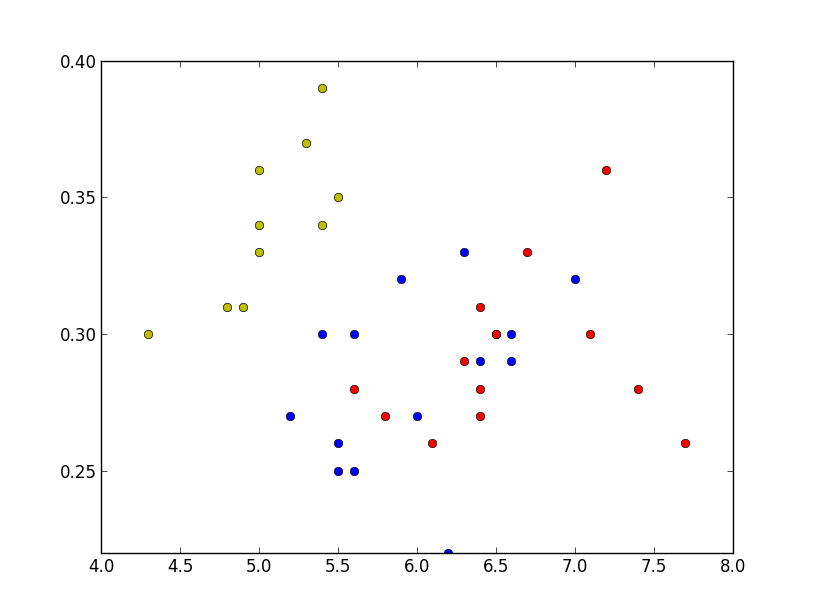
\includegraphics[width=\textwidth]{images/prob21-iristrain.png}
    \caption{Visualization of the iris training set.}
    \label{fig:iris_train}
\end{figure}

\begin{figure}[htbp]
    \centering
    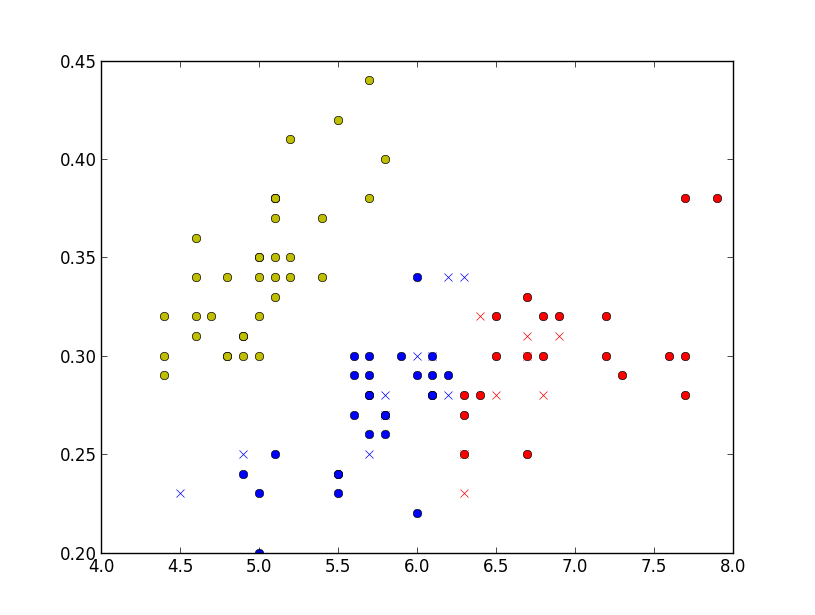
\includegraphics[width=\textwidth]{images/prob21-lda.png}
    \caption{Visualization of the iris testing set classified with the LDA.
             Crosses signify misclassified points.}
    \label{fig:iris_lda}
\end{figure}

\section{Question 2.2}

Using a $k$-NN classifier we can see a clear problem with the metric. Because
the width of the sepals is much smaller than the length, the nearest neighbours
are simply the ones with most similar width. This causes a lot of data points
to be misclassified. The more neighbours we considered, the more the sepal
length mattered. \autoref{fig:knn_std} shows the classifications given using
$5$-NN. It is quite clear (see the blue crosses in the top, and yellow ones in
the bottom), that the sepal width means too much for the $k$-NN classifier.
The error rates were $34\%$ for $1$-NN, $27\%$ for $3$-NN, $23\%$ for $5$-NN,
and $23\%$ for $7$-NN.

\begin{figure}[htbp]
    \centering
    \caption{Visualization of the $5$-NN classification of the iris test set
    using the $l_2$ norm. Triangles indicate training points. circles indicate
    correctly classified test points, and crosses indicate incorrectly classified
    test points.}
    \label{fig:knn_std}
\end{figure}


\section{Question 2.3}
We are given the function $d : \mathbb{R}^2 \times \mathbb{R}^2 \rightarrow \mathbb{R}$ defined as
$$d(\bm{x},\bm{z}) = \| \bm{Mx} - \bm{Mz} \|_{2} = \| \bm{M}(\bm{x} - \bm{z}) \|_{2}$$

where
$$\bm{M} = \begin{pmatrix} 1 & 0 \\ 0 & 10 \end{pmatrix}$$

and $\bm{x},\bm{y} \in \mathbb{R}^2$. In order to be a metric, the function $d$ must satisfy the following conditions:

\begin{enumerate}
    \item $d(\bm{x},\bm{z}) \geq 0$
    \item $d(\bm{x},\bm{z}) = 0$\ \ \ iff $x = z$
    \item $d(\bm{x},\bm{z}) = d(\bm{z},\bm{x})$
    \item $d(\bm{x},\bm{z}) \leq d(\bm{x},\bm{y}) + d(\bm{y},\bm{z})$
\end{enumerate}

All of the conditions follow directly from the definition of a norm, which has the
following properties:

\begin{enumerate}
    \setcounter{enumi}{4}
    \item $\| a\bm{x}\| = |a|\| \bm{x} \|$\ \ where $a \in \mathbb{R}$
    \item $\| \bm{x} \| \geq 0$
    \item $\| \bm{x} \| = 0$\ \ \ iff $\bm{x} = 0$
    \item $\| \bm{x} + \bm{y} \| \leq \| \bm{x} \| + \| \bm{y} \|$
\end{enumerate}

Because $d$ is a norm, it is trivial that $(1)$ follows from $(6)$ and $(2)$ follows from $(7)$. Because of $(5)$ we get that 

\begin{align*}
    d(\bm{x}, \bm{z}) &= \| \bm{M}(\bm{x} - \bm{z}) \|_{2} \\
                      &= \| \bm{M}(-1\cdot(\bm{z} - \bm{x})) \|_{2} \\
                      &= |-1|\| \bm{M}(\bm{z} - \bm{x}) \|_{2} \tag{per 5}\\
                      &= \| \bm{M}(\bm{z} - \bm{x}) \|_{2} \\
                      &= d(\bm{z},\bm{x})
\end{align*}

which implies $(3)$. Finally, we need to check $(4)$ where we use

\begin{align*}
d(\bm{x}, \bm{y}) + 
d(\bm{y}, \bm{z}) &= \| \bm{M}(\bm{x} - \bm{y}) \|_{2} + \| \bm{M}(\bm{y} - \bm{z}) \|_{2} \\
                  &\geq \| \bm{M}(\bm{x} - \bm{y}) +  \bm{M}(\bm{y} - \bm{z}) \|_{2} \tag{per 8}\\
                  &= \| \bm{M}(\bm{x} - \bm{z}) \|_{2} \\
                  &= d(\bm{x},\bm{z})
\end{align*}
\qed


\section{Question 2.4}
As already mentioned under question 2.2, the $l_2$ norm is heavily skewed
towards the sepal width compared to the sepal length. This resulted in bad
classifications earlier. If we use the metric from question 2.3, we see, that
it effectively stretches the sepal-axis by a factor of $10$ to make the
distance calculations less skewed. Using the new metric we obtained error rates
of $24\%$, $24\%$, $22\%$, and $21\%$ respectively. \autoref{fig:knn_metr}
displays the classification using $7$-NN.

\begin{figure}[htbp]
    \centering
    \caption{Results of using the $7$-NN classifier on the iris test set with
    the new metric. Triangles indicate training points. circles indicate
    correctly classified test points, and crosses indicate incorrectly classified
    test points.}
    \label{fig:knn_metr}
\end{figure}

\section{Question 2.5}
Using the transformed data we get the exact same error rates ($8/38$ and
$18/100$). This is because stretching the data along one axis does not affect
the linear discriminant. It is merely a rescaling of all the $x_2$-coordinates.



\begin{thebibliography}{9}
    \bibitem{Bishop}
        C. M. Bishop,
        \emph{Pattern Recognition and Machine Learning},
        Springer Verlag,
        2006.
\end{thebibliography}

\end{document}
